% Created 2023-09-12 Tue 16:47
% Intended LaTeX compiler: pdflatex
\documentclass[11pt]{article}
\usepackage[utf8]{inputenc}
\usepackage[T1]{fontenc}
\usepackage{graphicx}
\usepackage{longtable}
\usepackage{wrapfig}
\usepackage{rotating}
\usepackage[normalem]{ulem}
\usepackage{amsmath}
\usepackage{amssymb}
\usepackage{capt-of}
\usepackage{hyperref}
\usepackage{siunitx, gensymb, tikz, pgfplots}
\author{Hankertrix}
\date{\today}
\title{Kinematics Tutorial}
\hypersetup{
 pdfauthor={Hankertrix},
 pdftitle={Kinematics Tutorial},
 pdfkeywords={},
 pdfsubject={},
 pdfcreator={Emacs 29.1 (Org mode 9.6.6)}, 
 pdflang={English}}
\begin{document}

\maketitle
\setcounter{tocdepth}{2}
\tableofcontents

\newpage

\section{Question 1}
\label{sec:orgd2447eb}

\subsection{(a)}
\label{sec:org349bb8f}

Let \(u_r\) be the initial velocity of the rock and \(u_b\) be the initial velocity of the ball.
\\[0pt]

At the time the ball and the rock collide, their displacement is the same, hence:

\[u_rt + \frac{1}{2}at^2 = u_b(t - 1) + \frac{1}{2}a(t - 1)^2\]
\[12t + \frac{1}{2}(-9.81)t^2 = 18(t - 1) + \frac{1}{2}(-9.81)(t - 1)^2\]
\[24t + (-9.81)t^2 = 36t - 36 + (-9.81)(t - 1)^2\]
\[9.81((t - 1)^2 - t^2) = 12t - 36\]
\[9.81(t^2 - 2t + 1 - t^2) = 12t - 36\]
\[9.81 - 19.62t = 12t - 36\]
\[31.62t = 45.81\]
\[t = \qty{1.45}{s} \text{ (3.s.f)}\]

\begin{center}
Thus, the ball and the rock will collide at \qty{1.45}{s}.
\end{center}


\subsection{(b)}
\label{sec:org3ad183e}

Solving for the displacement of the rock:

\[s = ut + \frac{1}{2}at^2\]
\[s = 12(1.45) + \frac{1}{2}(-9.81)(1.45)^2\]
\[s = \qty{7.10}{m} \text{ (3.s.f)}\]

\begin{center}
Thus, the ball and the rock will collide at a height of $\qty{7.10}{m}$.
\end{center}


\subsection{(c)}
\label{sec:orgd2069ec}

Let \(u_r\) be the initial velocity of the rock and \(u_b\) be the initial velocity of the ball.
\\[0pt]

At the time the ball and the rock collide, their displacement is the same, hence:

\[u_bt + \frac{1}{2}at^2 = u_r(t - 1) + \frac{1}{2}a(t - 1)^2\]
\[18t + \frac{1}{2}(-9.81)t^2 = 12(t - 1) + \frac{1}{2}(-9.81)(t - 1)^2\]
\[36t + (-9.81)t^2 = 24t - 24 + (-9.81)(t - 1)^2\]
\[9.81((t - 1)^2 - t^2) = -12t - 24\]
\[9.81(t^2 - 2t + 1 - t^2) = -12t - 24\]
\[9.81 - 19.62t = -12t - 24\]
\[7.62t = 33.81\]
\[t = \qty{4.44}{s} \text{ (3.s.f)}\]
\\[0pt]

Solving for the displacement of the ball:

\[s = ut + \frac{1}{2}at^2\]
\[s = 18(4.44) + \frac{1}{2}(-9.81)(4.44)^2\]
\[s = \qty{-16.7}{m} \text{ (3.s.f)}\]

Since the displacement of the ball is negative, that means the rock and the ball collide below the ground, which means that they did not collide.


\section{Question 2}
\label{sec:org5024be6}

\subsection{(a)}
\label{sec:org038da3b}

\[a = \frac{dv}{dt} = g - kv\]
\[\frac{\frac{dv}{dt}}{g - kv} = 1\]

\begin{equation}
\int \frac{\frac{dv}{dt}}{g - kv} \,dt = \int 1 \,dt \tag{1}
\end{equation}

Let \(u = g - kv\). Differentiating \(u\) with respect to \(v\):

\begin{equation}
\frac{du}{dv} = - k \tag{2}
\end{equation}

Substituting \((2)\) into \((1)\) and multiplying \((1)\) by \(\frac{du}{dv}\):

\[\int \frac{1}{u} \, du = \int -k \, dt\]
\[\ln|u| = - kt + c, \text{ where c is an arbitrary constant}\]
\[u = e^{-kt + c}\]

Let \(B = e^c\), where \(B\) is an arbitrary constant:
\[u = Be^{-kt}\]

Substituting \(u = g - kv\) into \(u = Be^{-kt}\):
\[g - kv = Be^{-kt}\]
\[- kv = Be^{-kt} - g\]

Let \(A = \frac{B}{g}\), where \(A\) is an arbitrary constant.
\[- kv = Age^{-kt} - g\]
\[kv = g(1 - Ae^{-kt})\]

\begin{equation}
v = \frac{g}{k}(1 - Ae^{-kt}) \tag{3}
\end{equation}

\newpage

Since the body is assumed to start from rest, at \(t = 0\), \(v = 0\). Substituting \(t = 0\) and \(v = 0\) into \((3)\):

\[0 = \frac{g}{k}(1 - Ae^{-k(0)})\]
\[0 = 1 - A\]
\[A = 1\]

Substituting \(A = 1\) into \((3)\):
\[v = \frac{g}{k}(1 - e^{-kt})\]

Thus, the velocity of the body is \(v = \frac{g}{k}(1 - e^{-kt})\).

\subsection{(b)}
\label{sec:org083eb07}

As \(t \rightarrow \infty, 1 - e^{-kt} \rightarrow 1\), hence:

\[v_{max} = \frac{g}{k}(1)\]
\[v_{max} = \frac{g}{k}\]


\section{Question 3}
\label{sec:org9d91cd0}

For the water to land \(\qty{2.5}{m}\) away, the horizontal component of the velocity must be able to cover the distance in time \(t\), hence:
\[s = v_0t + \frac{1}{2}at^2\]
\[2.5 = 6.5\cos(\theta)t\]
\begin{equation}
t = \frac{5}{13}\sec(\theta) \tag{1}
\end{equation}

\newpage

The vertical displacement of the ball must be 0 when it hits the ground, so:

\[s = v_0t + \frac{1}{2}at^2\]
\[0 = 6.5\sin(\theta)t + \frac{1}{2}(-9.81)t^2\]
\[6.5\sin(\theta)t = 4.905t^2\]
\[6.5\sin(\theta) = 4.905t\]

\begin{equation}
t = \frac{1300}{981}\sin(\theta) \tag{2}
\end{equation}

Substituting \((1)\) into \((2)\):

\[\left(\frac{5}{13}\sec(\theta)\right) = \frac{1300}{981}\sin(\theta)\]
\[\sin(\theta)\cos(\theta) = \frac{981}{3380}\]
\[2\sin(\theta)\cos(\theta) = \frac{981}{1690}\]
\[\sin(2\theta) = \frac{981}{1690}\]

\begin{align*}
2\theta &= \sin^{-1}\left(\frac{981}{1690}\right) &\text{or}&
&180 - 2\theta &= \sin^{-1}\left(\frac{981}{1690}\right) \\
2\theta &= 35.4838 &\text{or}&
&180 - 2\theta &= 35.4838 \\
\theta &= 17.7 \degree \text{ (3.s.f)} &\text{or}&
&\theta &= 72.3 \degree \text{ (3.s.f)}
\end{align*}

For angles of \(\theta < 90 \degree\), there are two angles that will correspond to the same \(\sin\) value, \(90 \degree - \theta\) and \(\theta\). Thus, there are 2 angles that will correspond to the same distance that the water will travel.

\newpage

The trajectory of the projectile at the two different angles are:
\\[0pt]

\begin{center}
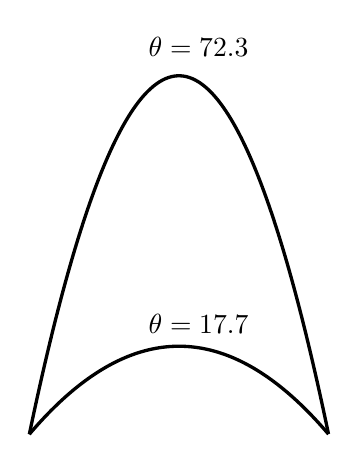
\begin{tikzpicture}
\draw[very thick, variable = \t, samples = 100, smooth, domain = 0:3.8]
    plot(\t, {1.2611 * (3.8 - \t) * \t}) node[above=140, left=25] {$\theta = 72.3$};
\draw[very thick, variable = \t, samples = 100, smooth, domain = 0:3.8]
    plot(\t, {0.30965 * (3.8 - \t) * \t}) node[above=40, left=25] {$\theta = 17.7$};
\end{tikzpicture}
\end{center}


\section{Question 4}
\label{sec:org21b0f3b}

\subsection{(a)}
\label{sec:orgb2225c1}

Let \(v_x\) and \(v_y\) be the initial velocity of the ball in the horizontal and vertical direction respectively. When the ball has reached the ground, the displacement of the ball in the vertical direction is \(\qty{-14.0}{m}\), thus:

\[s = v_yt + \frac{1}{2}at^2\]
\[-14 = -7\sin(40 \degree)t + \frac{1}{2}(-9.81)t^2\]
\[-28 = -14\sin(40 \degree)t - 9.81t^2 \]
\[9.81t^2 + 14\sin(40 \degree)t - 28 = 0\]

\begin{align*}
t &= -2.20926 &\text{or}& &t &= 1.29194 \\
t &= -2.21 \text{ (3.s.f)} &\text{or}& &t &= 1.29 \text{ (3.s.f)}
\end{align*}

Since time cannot be negative, \(t = \qty{1.29}{s}\).

\subsection{(b)}
\label{sec:orgedb44b7}

\(\indent\) The graph of \(x\) vs \(t\):
\\[0pt]

\begin{center}
\begin{tikzpicture}
\begin{axis}[xmin = 0, ymin = 0]
\addplot[color = black]{5.3623 * x};
\end{axis}
\end{tikzpicture}
\end{center}

The graph of \(y\) vs \(t\):
\\[0pt]

\begin{center}
\begin{tikzpicture}
\begin{axis}[xmin = 0, ymax = 0]
\addplot[color = black]{-4.49951 * x + (1/2) * (-9.81 * x^2)};
\end{axis}
\end{tikzpicture}
\end{center}

\newpage

The graph of \(v_x\) vs \(t\):
\\[0pt]

\begin{center}
\begin{tikzpicture}
\begin{axis}[xmin = 0, ymin = 0, ymax = 6]
\addplot[color = black]{5.3623};
\end{axis}
\end{tikzpicture}
\end{center}

The graph of \(v_y\) vs \(t\):
\\[0pt]

\begin{center}
\begin{tikzpicture}
\begin{axis}[xmin = 0, ymax = 0]
\addplot[color = black]{-4.49951 - 9.81 * x};
\end{axis}
\end{tikzpicture}
\end{center}

\newpage

\subsection{(c)}
\label{sec:org6f4a5c5}

Letting the displacement of the ball in the vertical direction be \(- 14 + 1.75 = \qty{-12.25}{m}\):

\[s = ut + \frac{1}{2}at^2\]
\[-12.25 = 7\sin(40 \degree)t + \frac{1}{2}(-9.81)t^2\]
\[-12.25 = 7\sin(40 \degree)t - 4.905t^2\]
\[4.905t^2 - 7\sin(40 \degree)t - 12.25 = 0\]

\begin{align*}
t &= 2.10421 &\text{or}& &t &= -1.18688 \\
t &= 2.10 \text{ (3.s.f)} &\text{or}& &t &= -1.19 \text{ (3.s.f)}
\end{align*}

Since time cannot be negative, \(t = \qty{2.10}{s}\). When \(t = \qty{2.10}{s}\), the horizontal displacement of the ball is:

\[s = ut + \frac{1}{2}at^2\]
\[s = 7\cos(40 \degree)(2.10)\]
\[s = 11.28342\]
\[s = \qty{11.3}{m}\]

Since the ball will be \(\qty{11.3}{m}\) away from the roof when it is \(\qty{1.75}{m}\) above the ground, the ball will not hit the man as he is only \(\qty{4}{m}\) away from the roof.


\section{Question 5}
\label{sec:orgf768e96}

The speed of the current will be equal to the east component of the boat's velocity. Thus, the speed of the current is \(3.4\sin(19.5 \degree) = \qty{1.134943}{m} = \qty{1.13}{ms^{-1}}\) (3.s.f).
\\[0pt]

The resultant speed of the boat with respect to the shore is \(3.4\cos(19.5 \degree) = 3.204981 = \qty{3.20}{ms^{-1}}\) (3.s.f).


\section{Question 6}
\label{sec:org832c937}

Let \(v_x\) be the component of the initial speed \(v_0\) that is parallel to the slope and \(v_y\) be the component of the initial speed that is perpendicular to the slope.
\[v_x = v_0 \cos(\theta - \phi)\]
\[v_y = v_0 \sin(\theta - \phi)\]
\\[0pt]

Let \(g_x\) be the component of the acceleration \(g\) that is parallel to the slope and \(g_y\) be the component of the acceleration \(g\) that is perpendicular to the slope.
\[g_x = g \sin(\phi) \tag{1}\]
\[g_y = g \cos(\phi) \tag{2}\]
\\[0pt]

Let \(t, \, t \neq 0\) be the time the ball takes to hit the ground again after being thrown. When the ball hits the ground again, the displacement of the ball must be 0.
\[s = ut + \frac{1}{2}at^2\]
\[0 = v_yt + \frac{1}{2}g_yt^2\]
\[0 = v_0 \sin(\theta - \phi)t - \frac{1}{2}g_yt^2\]
\[\frac{1}{2}g_yt = v_0 \sin(\theta - \phi)\]
\[g_yt = 2v_0 \sin(\theta - \phi)\]

\begin{equation}
t = \frac{2v_0 \sin(\theta - \phi)}{g_y} \tag{3}
\end{equation}
\\[0pt]

\newpage

The distance \(d\) travelled by the ball would be:
\[s = ut + \frac{1}{2}at^2\]
\[d = v_xt - \frac{1}{2}g_xt^2\]

\begin{equation}
d = v_0 \cos(\theta - \phi)t - \frac{1}{2}g_xt^2 \tag{4}
\end{equation}

Substituting \((3)\) into \((4)\):
\[d = v_0 \cos(\theta - \phi)\left(\frac{2v_0 \sin(\theta - \phi)}{g_y}\right) - \frac{1}{2}g_x\left(\frac{2v_0 \sin(\theta - \phi)}{g_y}\right)^2\]
\[d = \frac{2(v_0)^2 \sin(\theta - \phi) \cos(\theta - \phi)}{g_y} - \frac{4g_x(v_0)^2 \sin^2(\theta - \phi)}{2(g_y)^2}\]
\[d = \left(\frac{2(v_0)^2}{g_y}\right) \left(\sin(\theta - \phi) \cos(\theta - \phi) - \frac{g_x}{g_y}(\sin^2(\theta - \phi))\right) \tag{5}\]
\\[0pt]

Substituting \((1)\) and \((2)\) into \((5)\):
\[d = \left(\frac{2(v_0)^2}{g \cos(\phi)}\right) \left(\sin(\theta - \phi) \cos(\theta - \phi) - \frac{g \sin(\phi)}{g \cos(\phi)}(\sin^2(\theta - \phi))\right)\]
\[d = \left(\frac{2(v_0)^2 \sec(\phi)}{g}\right)(\sin(\theta - \phi) \cos(\theta - \phi) - \tan(\phi) \sin^2(\theta - \phi))\]
\[d = \left(\frac{2(v_0)^2 \sec(\phi)}{g}\right) \left(\frac{\sin(2(\theta - \phi))}{2} - \tan(\phi) \sin^2(\theta - \phi)\right)\]
\[d = \left(\frac{2(v_0)^2 \sec(\phi)}{g}\right) \left(\frac{\sin(2\theta - 2\phi)}{2} - \tan(\phi) \sin^2(\theta - \phi)\right)\]

\newpage

Differentiating \(d\) with respect to \(\theta\):
\[\frac{dd}{d\theta} = \left( \frac{2(v_0)^2 \sec(\phi)}{g}\right) (\cos(2\theta - 2\phi) - 2\tan(\phi) \sin(\theta - \phi) \cos(\theta - \phi))\]
\[\frac{dd}{d\theta} = \left( \frac{2(v_0)^2 \sec(\phi)}{g}\right) (\cos(2\theta - 2\phi) - \tan(\phi) \sin(2\theta - 2\phi))\]
\\[0pt]

When \(d\) is maximum, \(\frac{dd}{d\theta}\) is 0. Since \(\theta\) is always greater than \(\phi\), the point is a maximum point:

\[0 = \left(\frac{2(v_0)^2 \sec(\phi)}{g}\right) (\cos(2\theta - 2\phi) - \tan(\phi) \sin(2\theta - 2\phi))\]
\[0 = \cos(2\theta - 2\phi) - \tan(\phi) \sin(2\theta - 2\phi)\]
\[\cos(2\theta - 2\phi) = \tan(\phi) \sin(2\theta - 2\phi)\]
\[\cot(2\theta - 2\phi) = \tan(\phi)\]
\[\tan \left(\frac{\pi}{2} - (2\theta - 2\phi)\right) = \tan(\phi)\]
\[\tan \left(\frac{\pi}{2} - 2\theta + 2\phi \right) = \tan(\phi)\]
\[\frac{\pi}{2} - 2\theta + 2\phi = \phi\]
\[2\theta = \frac{\pi}{2} + \phi\]
\[\theta = \frac{\pi}{4} + \frac{\phi}{2}\]
\end{document}